\documentclass[4pt]{standalone}
\usepackage{tikz}
\usetikzlibrary{automata, positioning}
\usetikzlibrary{calc}
\usepackage{relsize}

\begin{document}
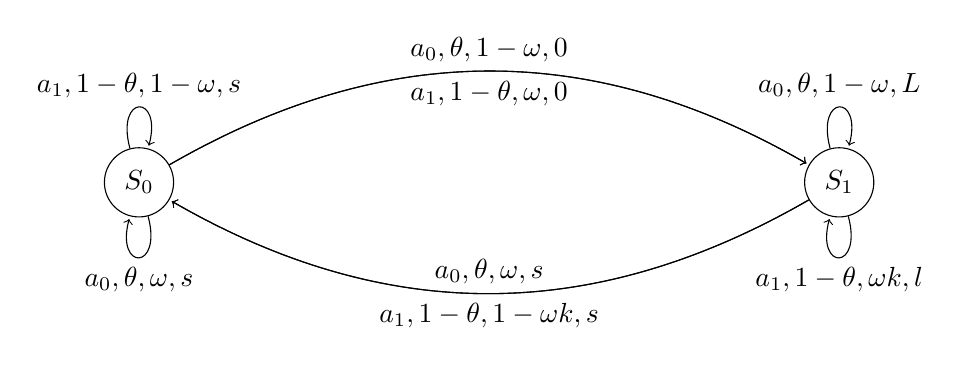
\begin{tikzpicture}
   % Drawing goes here
   \node[state] (s0) {$S_0$};
   \node[state, right = 8cm of s0] (s1) {$S_1$};
   % Connect the states with arrows
        \draw[every loop]
            (s0) edge[bend left, auto=left] node { $a_0, \theta,1-\omega, 0$} (s1)
            (s0) edge[loop below] node { $a_0,\theta,\omega, s$} (s0)
            (s0) edge[loop above] node { $a_1,1-\theta,1-\omega, s$} (s0)
            (s0) edge[bend left, auto=right] node { $a_1,1-\theta,\omega, 0$} (s1)
            (s1) edge[bend left, auto=right] node { $a_0, \theta, \omega, s$} (s0)
            (s1) edge[loop above] node{ $a_0, \theta, 1-\omega, L$} (s1)
            (s1) edge[loop below] node { $a_1,1-\theta,\omega k, l$} (s1)
            (s1) edge[bend left, auto=left] node { $a_1,1-\theta,1-\omega k, s$} (s0)
           ;
   
\end{tikzpicture}
\end{document}